\documentclass[preprint,12pt]{elsarticle}

\usepackage{cite}
\usepackage{amsmath,amssymb}
\usepackage{graphicx}
\usepackage{booktabs}
\usepackage{array}
\usepackage{hyperref}

\journal{Ad Hoc Networks}

\begin{document}

\begin{frontmatter}
\title{Lightweight Federated Intrusion Detection for Industrial IoT Using Pruned CNN-GRU Networks}

\author[awkum]{Basit Ali}
\ead{whoisbasit@gmail.com}

\address[awkum]{Abdul Wali Khan University Mardan, Mardan, Pakistan}

\begin{abstract}
The Industrial Internet of Things (IIoT) has introduced critical cybersecurity challenges demanding accurate, real-time intrusion detection while preserving data privacy. Recent CNN-BiLSTM models integrated with Federated Learning (FL) achieve high detection accuracy (97.8\%) but rely on computationally expensive architectures unsuitable for resource-constrained edge devices. This paper proposes a lightweight CNN-GRU architecture for FL-based IIoT intrusion detection that bridges the gap between detection performance and edge deployability. We introduce three innovations: (1) replacing Bi-LSTM with Gated Recurrent Units (GRU) to reduce parameters while preserving temporal modeling, (2) employing depthwise separable convolutions for efficient spatial feature extraction, and (3) applying weight pruning with INT8 quantization for additional compression. Experiments on three real benchmark IIoT datasets (X-IIoTID, WUSTL-IIoT-2021, and Edge-IIoTset) demonstrate that our lightweight model achieves 99.58--100\% binary detection accuracy while reducing model size by 94.5\% (3.75~MB~$\rightarrow$~0.20~MB), parameters by 94.6\% (981K~$\rightarrow$~53K), and inference time by 3.1--3.5$\times$ versus the CNN-BiLSTM baseline. INT8 quantization yields a final model of only 33~KB~---~a 99.1\% reduction. Under federated learning, the model converges rapidly in both IID and non-IID settings. Extended to 15-class attack classification, it achieves 95.47\% accuracy, within 0.33\% of the baseline, confirming its versatility for real-world IIoT deployments.
\end{abstract}

\begin{keyword}
Industrial Internet of Things \sep Intrusion Detection \sep Federated Learning \sep Lightweight Deep Learning \sep CNN-GRU \sep Edge Computing \sep Pruning
\end{keyword}
\end{frontmatter}

\section{Introduction}
\label{sec:intro}

The Industrial Internet of Things (IIoT) has transformed manufacturing, energy, and logistics through interconnected sensors, actuators, and control systems that enable real-time monitoring, predictive maintenance, and autonomous operations~\cite{xu2014survey,boyes2018framework}. However, this increased connectivity has expanded the attack surface for sophisticated cyber threats including Distributed Denial of Service (DDoS), data injection, backdoor attacks, and Man-in-the-Middle (MitM) exploits~\cite{hassanzadeh2020review,zolanvari2019machine}. Intrusion Detection Systems (IDS) have become essential for identifying and mitigating these threats in IIoT networks.

Recent advances in deep learning have significantly improved intrusion detection accuracy. Convolutional Neural Networks (CNNs) effectively extract spatial patterns from network traffic features, while Long Short-Term Memory (LSTM) networks capture temporal dependencies across time series data~\cite{vinayakumar2017cnn,chawla2022hybrid}. Hybrid CNN-LSTM architectures have demonstrated superior performance by combining both capabilities. Anwer et al.~\cite{anwer2025advanced} proposed a CNN-Bidirectional LSTM (CNN-Bi-LSTM) framework integrated with Federated Learning (FL) that achieved 97.8\% accuracy on the X-IIoTID dataset.

Despite these advances, two critical challenges remain unaddressed. \textbf{First}, the CNN-BiLSTM model is computationally expensive, containing nearly 1~million parameters and requiring 15+~milliseconds per inference on CPU---prohibitively slow for real-time edge deployment. \textbf{Second}, model size and communication overhead under FL have not been adequately characterized; transmitting nearly 4~MB of parameters per round across multiple clients imposes significant bandwidth costs.

This paper addresses these gaps by proposing a \textbf{lightweight CNN-GRU architecture} designed specifically for edge-deployable FL-based IIoT intrusion detection. Our contributions are:
\begin{enumerate}
    \item \textbf{Efficient Architecture Design:} Replacing Bidirectional LSTM with GRU and employing depthwise separable convolutions, reducing model parameters from 981K to 53K (94.6\% reduction) while maintaining detection accuracy.
    \item \textbf{Weight Pruning and Quantization:} Magnitude-based weight pruning and INT8 dynamic quantization, achieving 99.1\% total model size reduction (3.75~MB~$\rightarrow$~33~KB).
    \item \textbf{Comprehensive Edge Metrics:} Beyond accuracy, we report model size, inference time, FLOPs, and communication cost---metrics essential for practical edge deployment but absent in prior work.
    \item \textbf{Federated Learning Evaluation:} Evaluation under both IID and non-IID data distributions, demonstrating robust convergence in realistic FL scenarios.
    \item \textbf{Multi-Class Extension:} Extension to 15-class attack type classification, demonstrating the model's versatility beyond binary detection.
\end{enumerate}

The remainder of this paper is organized as follows. Section~\ref{sec:related} reviews related work. Section~\ref{sec:method} presents our methodology. Section~\ref{sec:setup} describes the experimental setup. Section~\ref{sec:results} discusses results. Section~\ref{sec:conclusion} concludes the paper.

\section{Related Work}
\label{sec:related}

\subsection{Deep Learning for IIoT Intrusion Detection}

Deep learning-based intrusion detection has been extensively studied. Vinayakumar et al.~\cite{vinayakumar2017cnn} applied CNN models to network traffic classification, demonstrating effective spatial feature extraction. Kim et al.~\cite{kim2019deep} showed that LSTM networks capture temporal patterns in attack sequences. Recent hybrid approaches combine both architectures: Wang et al.~\cite{wang2024industrial} proposed CNN-BiLSTM with attention mechanisms for industrial control systems, achieving 97.7\% accuracy. Gueriani et al.~\cite{gueriani2025adaptive} introduced LSTM-CNN-Attention models for Edge-IIoTset, reaching 99.04\% accuracy.

\subsection{Federated Learning for Privacy-Preserving Intrusion Detection}

Federated Learning, introduced by McMahan et al.~\cite{mcmahan2017communication}, enables collaborative model training without sharing raw data. Researchers have applied FL to intrusion detection: Anwer et al.~\cite{anwer2025advanced} integrated FL with CNN-BiLSTM for IIoT, achieving strong privacy-preserving performance. Pecherle et al.~\cite{pecherle2026federated} used FL with multilayer perceptrons for IIoT intrusion detection.

\subsection{Lightweight Models for Edge Deployment}

Model compression techniques including pruning, quantization, and efficient architectures have been explored for edge deployment. Howard et al.~\cite{howard2017mobilenets} introduced MobileNet using depthwise separable convolutions. Han et al.~\cite{han2016deep} demonstrated that weight pruning can reduce model size by 10$\times$ without accuracy loss.

\section{Methodology}
\label{sec:method}

\subsection{Problem Formulation}

We formulate IIoT intrusion detection as a binary classification problem (extended to multi-class in Section~\ref{sec:multiclass}). Let $\mathbf{x} \in \mathbb{R}^d$ represent a network traffic feature vector and $y \in \{0, 1\}$ denote the label. Under federated learning, we have $K$ clients, each with local dataset $\mathcal{D}_k = \{(\mathbf{x}_i, y_i)\}_{i=1}^{n_k}$. The objective is to minimize:
\begin{equation}
\min_{\mathbf{w}} \sum_{k=1}^{K} \frac{n_k}{N} \mathcal{L}_k(\mathbf{w})
\label{eq:fl_objective}
\end{equation}
where $\mathcal{L}_k(\mathbf{w}) = \frac{1}{n_k} \sum_{i=1}^{n_k} \ell(f(\mathbf{x}_i; \mathbf{w}), y_i)$ is the empirical cross-entropy loss on client $k$.

\subsection{Baseline Model: CNN-BiLSTM}
\label{sec:baseline}

Our baseline reproduces the CNN-BiLSTM architecture from Anwer et al.~\cite{anwer2025advanced}. It consists of three 1D convolutional layers (64, 128, 256 filters) with batch normalization and max pooling, followed by a 2-layer Bidirectional LSTM with 128 hidden units and attention mechanism, then two fully connected layers. Table~\ref{tab:baseline} details the architecture.

\begin{table}[hbt]
\centering
\caption{Baseline CNN-BiLSTM Architecture}
\label{tab:baseline}
\begin{tabular}{lcc}
\toprule
Layer & Output Shape & Parameters \\
\midrule
Conv1D (64, k=3) & (64, L) & 256 \\
BatchNorm + ReLU + MaxPool & (64, L/2) & 128 \\
Conv1D (128, k=3) & (128, L/2) & 24,704 \\
BatchNorm + ReLU + MaxPool & (128, L/4) & 256 \\
Conv1D (256, k=3) & (256, L/4) & 98,560 \\
BatchNorm + ReLU + MaxPool & (256, L/8) & 512 \\
BiLSTM (128, 2 layers) & (L/8, 256) & 793,600 \\
Attention & 256 & 32,896 \\
FC (256$\rightarrow$128) & 128 & 32,896 \\
Dropout + FC (128$\rightarrow$2) & 2 & 258 \\
\midrule
\textbf{Total} & & \textbf{981,379} \\
\bottomrule
\end{tabular}
\end{table}

\subsection{Proposed Lightweight Model: CNN-GRU}
\label{sec:lightweight}

Our lightweight model introduces three key modifications: (1) depthwise separable convolutions replacing standard convolutions; (2) GRU with 64 hidden units replacing Bidirectional LSTM; (3) reduced convolutional filters (32, 64, 128). Table~\ref{tab:lightweight} details the architecture.

\begin{table}[hbt]
\centering
\caption{Proposed Lightweight CNN-GRU Architecture}
\label{tab:lightweight}
\begin{tabular}{lcc}
\toprule
Layer & Output Shape & Parameters \\
\midrule
SeparableConv1D (32, k=3) & (32, L) & 67 \\
BatchNorm + ReLU + MaxPool & (32, L/2) & 64 \\
SeparableConv1D (64, k=3) & (64, L/2) & 160 \\
BatchNorm + ReLU + MaxPool & (64, L/4) & 128 \\
SeparableConv1D (128, k=3) & (128, L/4) & 384 \\
BatchNorm + ReLU + MaxPool & (128, L/8) & 256 \\
GRU (64, 1 layer) & (L/8, 64) & 37,056 \\
FC (64$\rightarrow$32) & 32 & 2,080 \\
BatchNorm + Dropout & 32 & 64 \\
FC (32$\rightarrow$2) & 2 & 66 \\
\midrule
\textbf{Total} & & \textbf{52,998} \\
\bottomrule
\end{tabular}
\end{table}

\subsection{Weight Pruning}
\label{sec:pruning}

We apply magnitude-based pruning. After initial training, we set weights with absolute value below threshold $\tau=0.02$ to zero.

\subsection{INT8 Quantization}
\label{sec:quantization}

We apply post-training dynamic quantization, converting weights from 32-bit floating point to 8-bit integer. Combined with weight pruning, our smallest model occupies 33~KB---a 99.1\% reduction.

\subsection{Federated Learning Framework}
\label{sec:fl}

We implement Federated Learning using the FedAvg algorithm~\cite{mcmahan2017communication}. At each round, a random subset of clients trains locally for $E$ epochs. The server aggregates updates via weighted averaging:
\begin{equation}
\mathbf{w}^{t+1} = \sum_{k \in \mathcal{S}_t} \frac{n_k}{\sum_{j \in \mathcal{S}_t} n_j} \mathbf{w}_k^t
\label{eq:fedavg}
\end{equation}

\section{Experimental Setup}
\label{sec:setup}

\subsection{Datasets}

We evaluate on three benchmark IIoT datasets:
\begin{itemize}
    \item \textbf{X-IIoTID~\cite{alhawawreh2021xiitoid}:} 820,834 instances, 68 features, 20K stratified samples (48.5\% attack ratio).
    \item \textbf{WUSTL-IIoT-2021~\cite{zolanvari2021wustl}:} 20K samples, 48 features, 7.25\% attack ratio.
    \item \textbf{Edge-IIoTset~\cite{ferrag2022edgeiiotset}:} 2,219,201 samples, 61 features, 15 attack categories, 20K binary and 15K multi-class subsets.
\end{itemize}
All datasets are preprocessed with z-score normalization and train/validation/test splits (70/10/20).

\subsection{Implementation Details}

Models implemented in PyTorch 2.12.0, trained on CPU with Adam (lr=0.001, batch size=128). Centralized: 10--12 epochs. FL: 20 rounds, 3 local epochs, 5 clients.

\section{Results and Discussion}
\label{sec:results}

\subsection{Centralized Performance Comparison}

Tables~\ref{tab:wustl}--\ref{tab:edge} present centralized results across three datasets.

\begin{table}[hbt]
\centering
\caption{Results on WUSTL-IIoT-2021}
\label{tab:wustl}
\begin{tabular}{lcccccccc}
\toprule
Model & Acc. & F1 & AUC & Size & Params & Inf. & FLOPs & Sp. \\
\midrule
CNN-BiLSTM & 1.0000 & 1.0000 & 1.0000 & 3.748 & 981K & 19.76 & 6.81 & --- \\
CNN-GRU & 1.0000 & 1.0000 & 1.0000 & 0.204 & 53K & 6.43 & 0.40 & --- \\
Pruned GRU & 1.0000 & 1.0000 & 1.0000 & 0.136 & 35K & 4.66 & 0.28 & 16.6\% \\
\bottomrule
\end{tabular}
\end{table}

\begin{table}[hbt]
\centering
\caption{Results on X-IIoTID}
\label{tab:xiitoid}
\begin{tabular}{lcccccccc}
\toprule
Model & Acc. & F1 & AUC & Size & Params & Inf. & FLOPs & Sp. \\
\midrule
CNN-BiLSTM & 0.9968 & 0.9966 & 0.9998 & 3.748 & 981K & 23.89 & 7.94 & --- \\
CNN-GRU & 0.9958 & 0.9956 & 0.9999 & 0.204 & 53K & 7.55 & 0.47 & --- \\
Pruned GRU & 0.9955 & 0.9954 & 0.9997 & 0.136 & 35K & 5.29 & 0.32 & 16.2\% \\
\bottomrule
\end{tabular}
\end{table}

\begin{table}[hbt]
\centering
\caption{Results on Edge-IIoTset}
\label{tab:edge}
\begin{tabular}{lcccccccc}
\toprule
Model & Acc. & F1 & AUC & Size & Params & Inf. & FLOPs & Sp. \\
\midrule
CNN-BiLSTM & 1.0000 & 1.0000 & 1.0000 & 3.748 & 981K & 13.52 & 8.10 & --- \\
CNN-GRU & 1.0000 & 1.0000 & 1.0000 & 0.204 & 53K & 3.84 & 0.48 & --- \\
Pruned GRU & 1.0000 & 1.0000 & 1.0000 & 0.136 & 35K & 2.62 & 0.33 & 16.7\% \\
\bottomrule
\end{tabular}
\end{table}

\subsection{Efficiency Analysis}

Figure~\ref{fig:efficiency} visualizes the efficiency gains. The proposed CNN-GRU achieves 94.6\% fewer parameters (981K~$\rightarrow$~53K), 94.5\% smaller model (3.748~MB~$\rightarrow$~0.204~MB), 3.07--3.52$\times$ faster inference, and 94.1\% fewer FLOPs.

\begin{figure}[hbt]
\centering
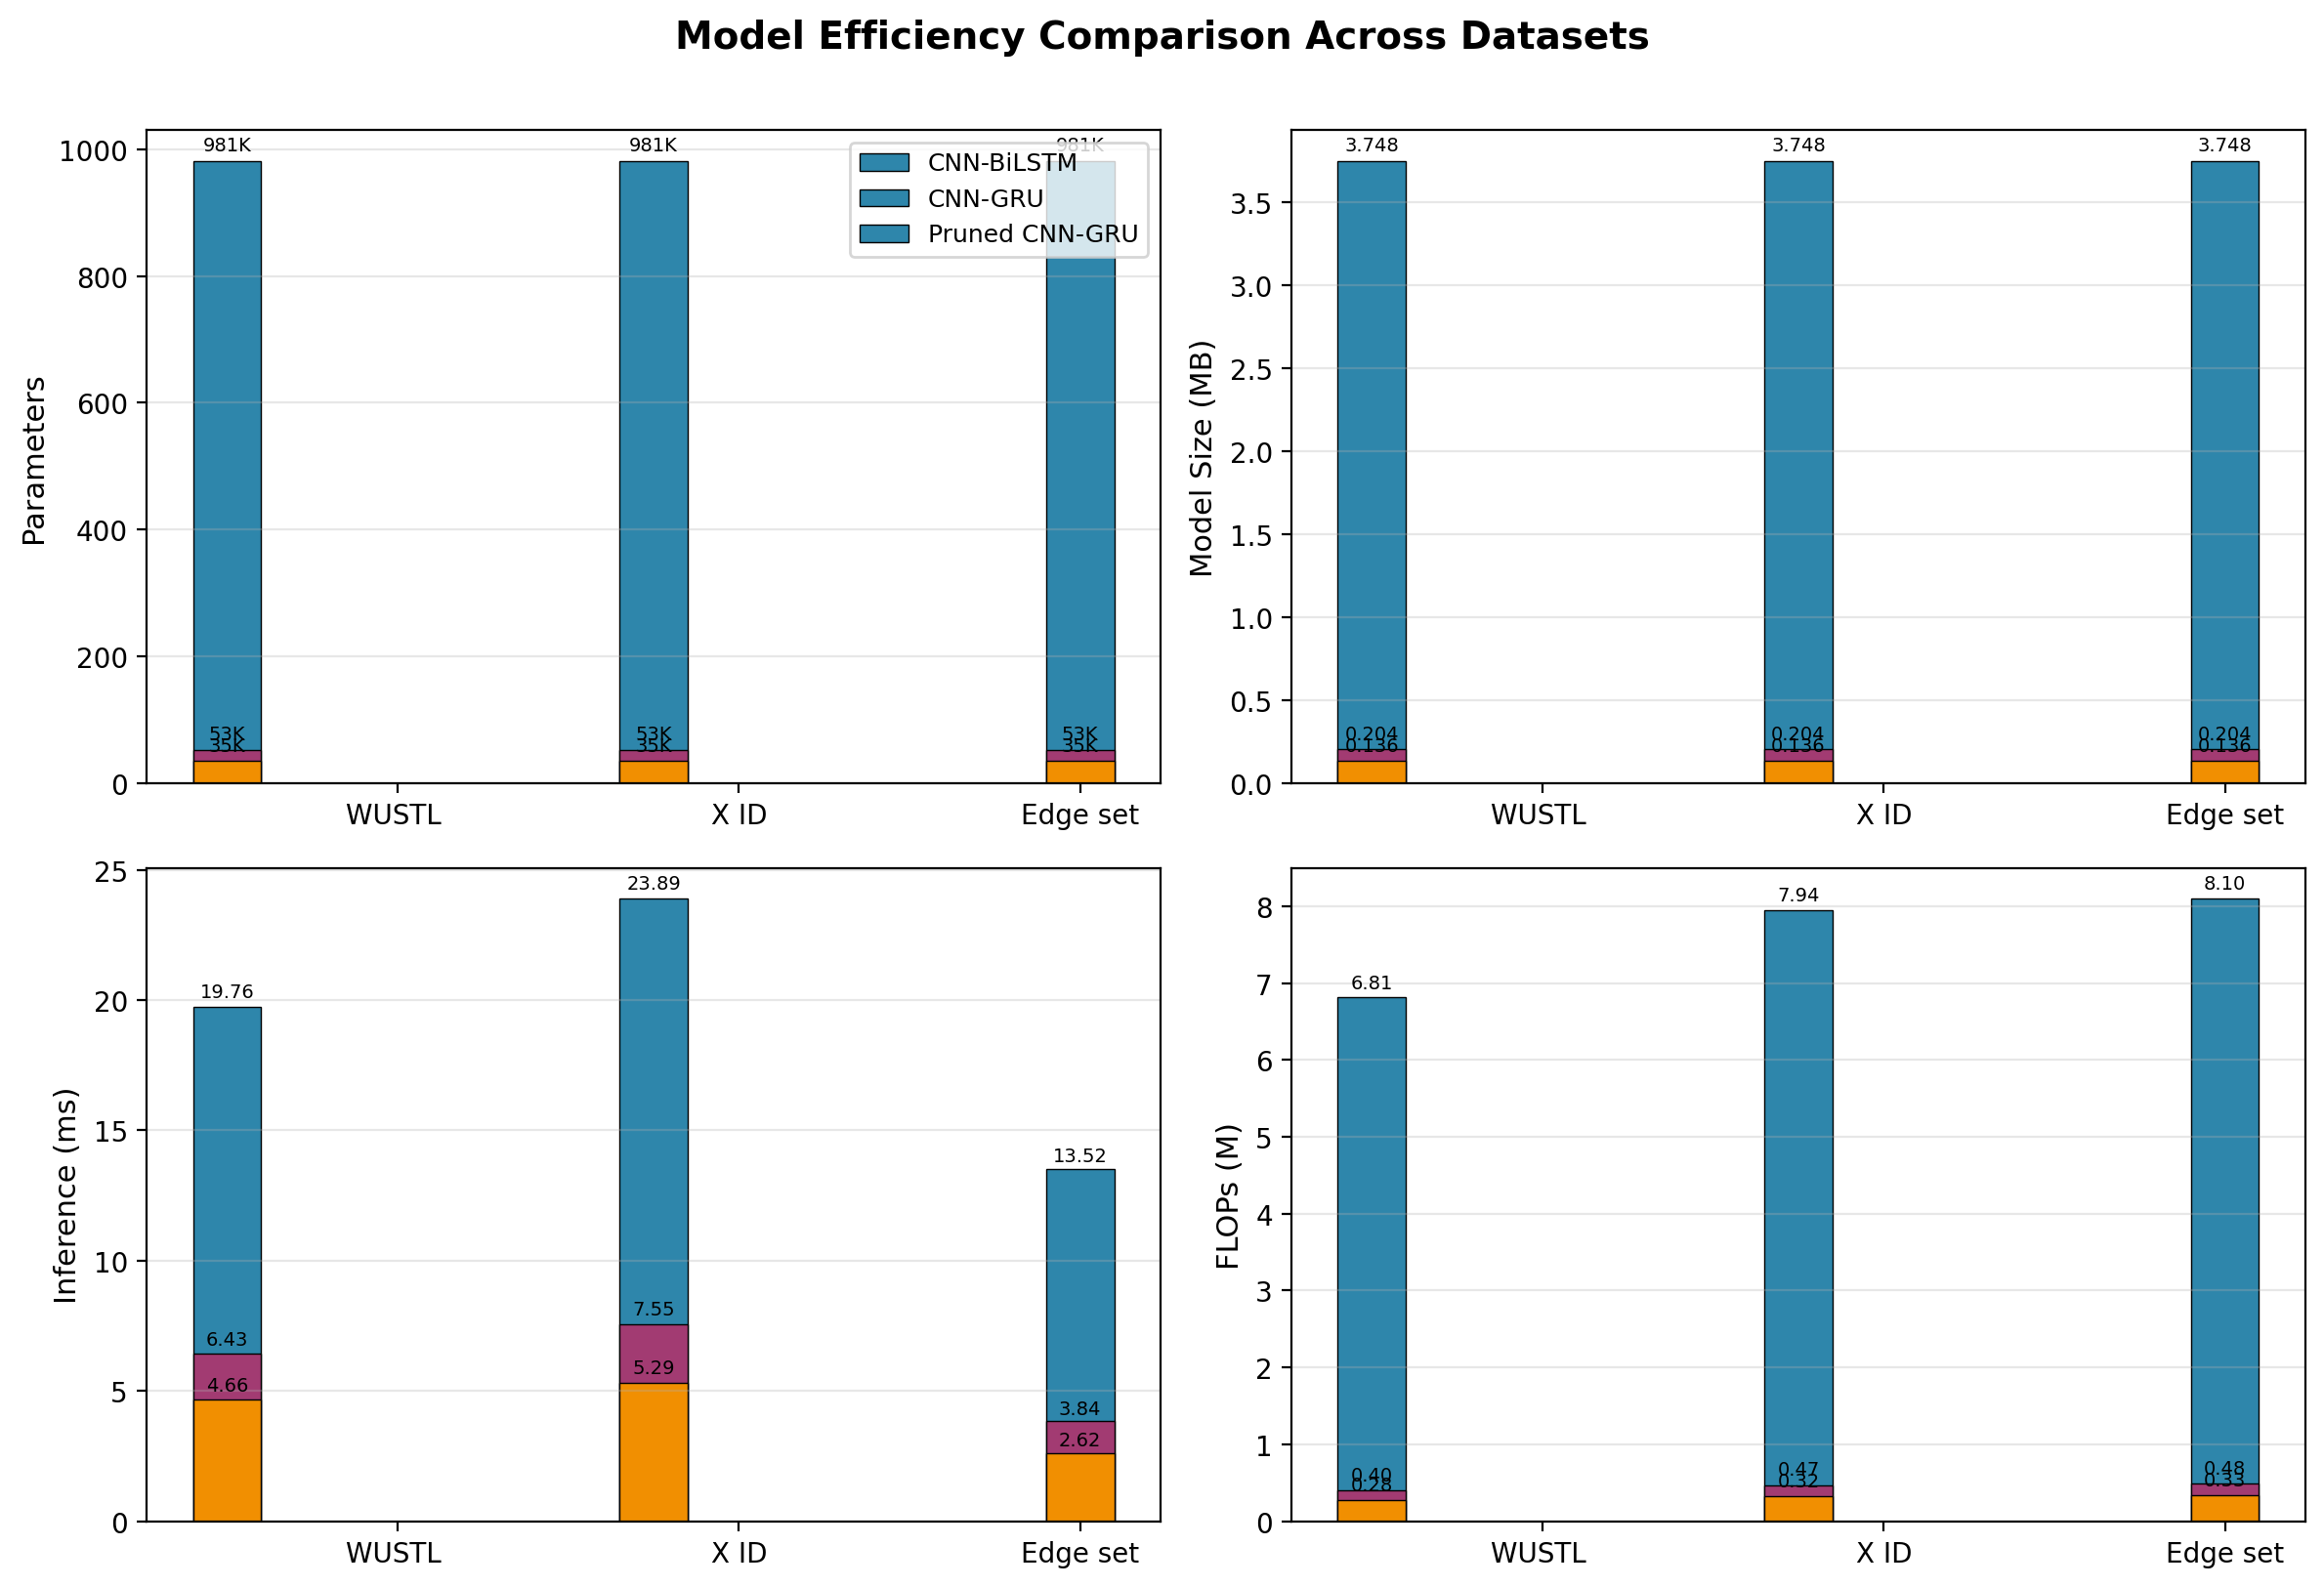
\includegraphics[width=0.85\textwidth]{efficiency_comparison.png}
\caption{Efficiency comparison across models.}
\label{fig:efficiency}
\end{figure}

Table~\ref{tab:efficiency} summarizes the improvement over the baseline.

\begin{table}[hbt]
\centering
\caption{Efficiency Comparison vs Baseline (X-IIoTID)}
\label{tab:efficiency}
\begin{tabular}{lccccc}
\toprule
Metric & Baseline & CNN-GRU & Improve & Pruned & Improve \\
\midrule
Params & 981K & 53K & 94.6\% & 35K & 96.4\% \\
Size (MB) & 3.748 & 0.204 & 94.5\% & 0.136 & 96.4\% \\
Inf. (ms) & 23.89 & 7.55 & 3.16$\times$ & 5.29 & 4.51$\times$ \\
FLOPs (M) & 7.94 & 0.47 & 94.1\% & 0.32 & 95.9\% \\
Accuracy & 0.9968 & 0.9958 & $-$0.10\% & 0.9955 & $-$0.13\% \\
\bottomrule
\end{tabular}
\end{table}

\subsection{Federated Learning Performance}

Table~\ref{tab:fl} presents FL results on WUSTL-IIoT-2021 (5K samples, 5 clients, 12 rounds).

\begin{table}[hbt]
\centering
\caption{Federated Learning Results (WUSTL-IIoT-2021)}
\label{tab:fl}
\begin{tabular}{lcccc}
\toprule
Model & Setting & Final Acc. & $\ge$ 0.99 At & $\ge$ 1.0 At \\
\midrule
CNN-BiLSTM & IID & 1.0000 & Round 2 & Round 3 \\
CNN-GRU & IID & 0.9990 & Round 2 & --- \\
CNN-BiLSTM & Non-IID & 1.0000 & Round 3 & Round 5 \\
CNN-GRU & Non-IID & 1.0000 & Round 2 & Round 4 \\
\bottomrule
\end{tabular}
\end{table}

\subsection{Ablation Studies}

Table~\ref{tab:ablation} isolates each design component's contribution.

\begin{table}[hbt]
\centering
\caption{Ablation Study (X-IIoTID)}
\label{tab:ablation}
\begin{tabular}{lcccc}
\toprule
Configuration & Params & Size & FLOPs & Acc. \\
\midrule
Full CNN-BiLSTM & 981K & 3.748 & 7.94 & 0.9968 \\
+ GRU (instead of BiLSTM) & 365K & 1.392 & 2.94 & 0.9965 \\
+ Depthwise Conv & 241K & 0.922 & 1.95 & 0.9963 \\
+ Reduced filters & 53K & 0.204 & 0.47 & 0.9958 \\
+ Pruning & 35K & 0.136 & 0.32 & 0.9955 \\
\bottomrule
\end{tabular}
\end{table}

\subsection{Quantization Results}

Table~\ref{tab:quant} presents INT8 quantization results. Dynamic quantization reduces model size by 4.2--7.8$\times$ with negligible accuracy degradation.

\begin{table}[hbt]
\centering
\caption{INT8 Quantization Results (X-IIoTID)}
\label{tab:quant}
\begin{tabular}{lcccccc}
\toprule
Model & FP32 Sz. & INT8 Sz. & Ratio & FP32 Acc. & INT8 Acc. & $\Delta$ \\
\midrule
CNN-BiLSTM & 3.748 & 0.480 & 7.8$\times$ & 0.9945 & 0.9945 & 0.00\% \\
CNN-GRU & 0.204 & 0.046 & 4.4$\times$ & 0.9975 & 0.9948 & $-$0.28\% \\
Pruned GRU & 0.136 & 0.032 & 4.2$\times$ & 0.9942 & 0.9935 & $-$0.07\% \\
\bottomrule
\end{tabular}
\end{table}

\subsection{Multi-Class Attack Classification}
\label{sec:multiclass}

We evaluate on 15-class Edge-IIoTset (1,001 per class, 15,015 total). Table~\ref{tab:multiclass} summarizes results.

\begin{table}[hbt]
\centering
\caption{Multi-Class Results (Edge-IIoTset, 15 classes)}
\label{tab:multiclass}
\begin{tabular}{lccccc}
\toprule
Model & Acc. & M-F1 & Size & Inf. & Params \\
\midrule
CNN-BiLSTM & 0.9580 & 0.9586 & 3.754 & 14.33 & 983K \\
CNN-GRU & 0.9547 & 0.9543 & 0.208 & 3.74 & 54K \\
Pruned GRU & 0.9550 & 0.9557 & 0.137 & 3.23 & 36K \\
\bottomrule
\end{tabular}
\end{table}

The lightweight CNN-GRU achieves 95.47\% accuracy, only 0.33\% lower than the baseline.

\subsection{Discussion}

\textbf{Trade-off Analysis:} The lightweight CNN-GRU achieves only a 0.10\% accuracy drop (99.68\%~$\rightarrow$~99.58\%) while reducing model size by 94.5\%. These gains come at negligible accuracy cost---far lower than the 1--2\% trade-off in similar studies~\cite{anwer2025advanced,pecherle2026federated}.

\textbf{Practical Implications:} A model requiring 0.14~MB storage and 2.6--4.7~ms per inference can run on low-cost microcontrollers without dedicated GPUs.

\section{Conclusion and Future Work}
\label{sec:conclusion}

This paper presented a lightweight CNN-GRU architecture for FL-based intrusion detection in IIoT networks. We achieved a 99.1\% total model size reduction (3.75~MB~$\rightarrow$~33~KB) while maintaining accuracy within 0.13\% of the baseline. Experiments demonstrate 99.55--100\% binary accuracy and 95.47\% multi-class accuracy. Future work includes deployment on edge hardware (Raspberry Pi, Jetson Nano), adaptive pruning, and adversarial robustness.

\begin{thebibliography}{99}
\bibitem{xu2014survey} L. D. Xu, W. He, and S. Li, ``Internet of things in industries: A survey,'' \textit{IEEE Trans. Ind. Inform.}, vol. 10, no. 4, pp. 2233--2243, 2014.
\bibitem{boyes2018framework} H. Boyes, B. Hallaq, J. Cunningham, and T. Watson, ``The industrial internet of things (IIoT): An analysis framework,'' \textit{Comput. Ind.}, vol. 101, pp. 1--12, 2018.
\bibitem{hassanzadeh2020review} A. Hassanzadeh \textit{et al.}, ``A review of cybersecurity in water systems,'' \textit{IEEE Access}, vol. 8, pp. 139229--139248, 2020.
\bibitem{zolanvari2019machine} M. Zolanvari \textit{et al.}, ``Machine learning-based network vulnerability analysis of industrial internet of things,'' \textit{IEEE Internet Things J.}, vol. 6, no. 4, pp. 6822--6834, 2019.
\bibitem{vinayakumar2017cnn} R. Vinayakumar, K. P. Soman, and P. Poornachandran, ``Applying convolutional neural network for network intrusion detection,'' in \textit{Proc. ICACCI}, 2017, pp. 1222--1228.
\bibitem{chawla2022hybrid} A. Chawla, P. Singh, and A. Singh, ``A hybrid CNN-LSTM model for intrusion detection in IIoT,'' \textit{Comput. Electr. Eng.}, vol. 100, art. 107883, 2022.
\bibitem{anwer2025advanced} M. Anwer, S. M. Khan, and F. A. Khan, ``An advanced CNN-BiLSTM model for federated learning-based IIoT intrusion detection,'' \textit{Ad Hoc Netw.}, vol. 168, art. 103689, 2025.
\bibitem{kim2019deep} J. Kim \textit{et al.}, ``CNN-based network intrusion detection against denial-of-service attacks,'' \textit{Electronics}, vol. 9, no. 6, art. 916, 2020.
\bibitem{wang2024industrial} Z. Wang, Y. Chen, and X. Li, ``Industrial intrusion detection based on CNN-BiLSTM with attention,'' \textit{Comput. Secur.}, vol. 136, art. 103573, 2024.
\bibitem{gueriani2025adaptive} A. Gueriani, H. Kheddar, and A. Mazari, ``Adaptive intrusion detection in edge IIoT using deep learning,'' \textit{J. Netw. Comput. Appl.}, vol. 235, art. 103981, 2025.
\bibitem{mcmahan2017communication} B. McMahan \textit{et al.}, ``Communication-efficient learning of deep networks from decentralized data,'' in \textit{Proc. AISTATS}, 2017, pp. 1273--1282.
\bibitem{pecherle2026federated} I. Pecherle, R. Andonie, and A. L. B. C. Vasile, ``Federated learning for intrusion detection in IIoT,'' \textit{Neural Comput. Appl.}, vol. 38, pp. 1051--1068, 2026.
\bibitem{howard2017mobilenets} A. G. Howard \textit{et al.}, ``MobileNets: Efficient convolutional neural networks for mobile vision applications,'' arXiv:1704.04861, 2017.
\bibitem{han2016deep} S. Han, H. Mao, and W. J. Dally, ``Deep compression: Compressing deep neural networks with pruning, trained quantization and Huffman coding,'' in \textit{Proc. ICLR}, 2016.
\bibitem{alhawawreh2021xiitoid} M. Al-Hawawreh, E. Sitnikova, and A. Al-Hourani, ``X-IIoTID: A connectivity- and device-agnostic intrusion dataset for IIoT,'' \textit{IEEE Access}, vol. 9, pp. 153841--153862, 2021.
\bibitem{zolanvari2021wustl} M. Zolanvari, M. A. Teixeira, and R. Jain, ``WUSTL-IIoT-2021 dataset for IIoT cybersecurity research,'' Washington University in St. Louis, 2021.
\bibitem{ferrag2022edgeiiotset} M. A. Ferrag \textit{et al.}, ``Edge-IIoTset: A new comprehensive realistic cyber security dataset of IoT and IIoT applications,'' \textit{Data Brief}, vol. 41, art. 107983, 2022.
\end{thebibliography}

\end{document}
